\chapter{Modelling the impact of dopamine on PY neurons}
\label{chap:modelling}
\section{Introduction}
\label{sec:model}

The Hodgkin-Huxley model is a conductance based, mathematical model that describes how action potentials in neurons are initiated and propagated. The model comprise four differential equations that were described in detail in Chapter \ref{chap:background} section \ref{sec:hogkin_huxley_model}. The original model included only potassium, sodium and leak currents. However, the model is relatively easily extensible to include several more channels and can also be adapted to create multi-compartmental representations of neurons. Each compartment is modelled with its own set of differential equations. The major challenge with this approach is the selection of parameter values and ranges finding a differential equation solver that can cope with the stiffness of the equations. Individual neuron models can be connected through model synapses to create a circuit.

\section{The Model}

In this chapter an implementation of the Hodgkin-Huxley model is presented to include five \acp{PY}, two \acp{PD}, one \ac{AB} and one \ac{LP} (fig. \ref{fig:HH_model}). Each of the neurons is modelled with two compartments, one representing the primary neurite and dendrites (A) and the other representing the soma (S) (fig. \ref{fig:two_compartment}). The A compartments are responsible for producing action potentials while the S compartments produce slow wave oscillations. 

The model has been implemented in \matlab, using the ode45 method which is based on an explicit Runge-Kutta (4,5) formula. Several of the differential equation solvers available in \matlab were tested but ode45 was the only method that would not diverge to infinity. Simulations were performed on PCs with Linux and Windows operating systems as well as on a high performance cluster.

\matlab, R and Neuron were evaluated for creating the model. The decision to use \matlab was made because Neuron was found to diverge to infinity after only a few seconds of simulation with only a simplistic model and in R all ode solvers were tested but were also found to diverge to infinity and no results could be obtained. 

\begin{figure}[H]
	\begin{center}
		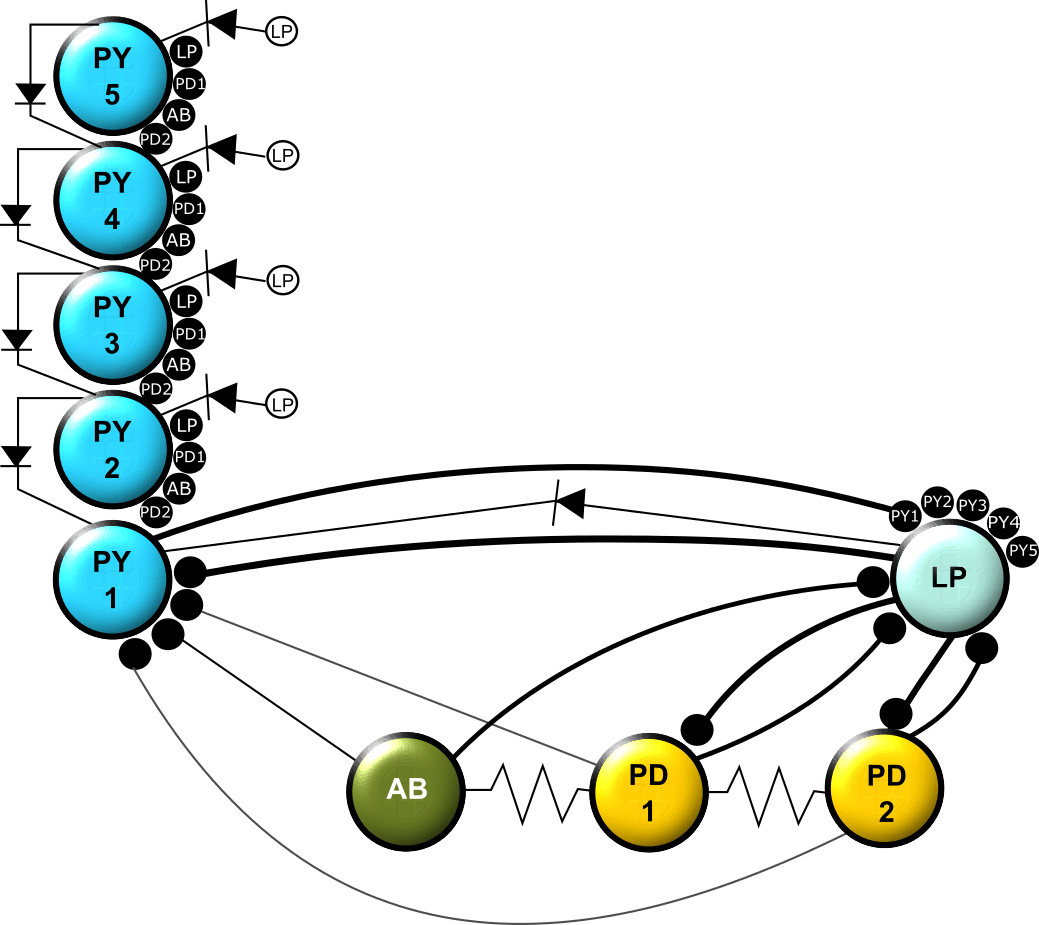
\includegraphics[width=10cm]{graphics/HH_model.png}
		\caption[Neural circuit of the pyloric \ac{CPG}.]{\textbf{Neural circuit of the pyloric \ac{CPG}. }The neural circuit of the model includes five \acp{PY}, two \acp{PD}, one \ac{AB} and one \ac{LP}. Neurons are shown with large coloured circles. All known inhibitory and electrical synapses are included in the model. The inhibitory synapses are shown as small black circles. Rectifying gap junctions are shown as diode symbols and non-rectifying gap junctions are indicated with resistor symbols. For clarity not all synapses and gap junctions in diagram are connected but the name of the inhibiting neuron is shown in the black circle. Similarly, not all the electrical synapses are connected but the name of the originating neuron is shown in a clear circle.}
		\label{fig:HH_model}
	\end{center}
\end{figure}

\begin{figure}[H]
	\begin{center}
		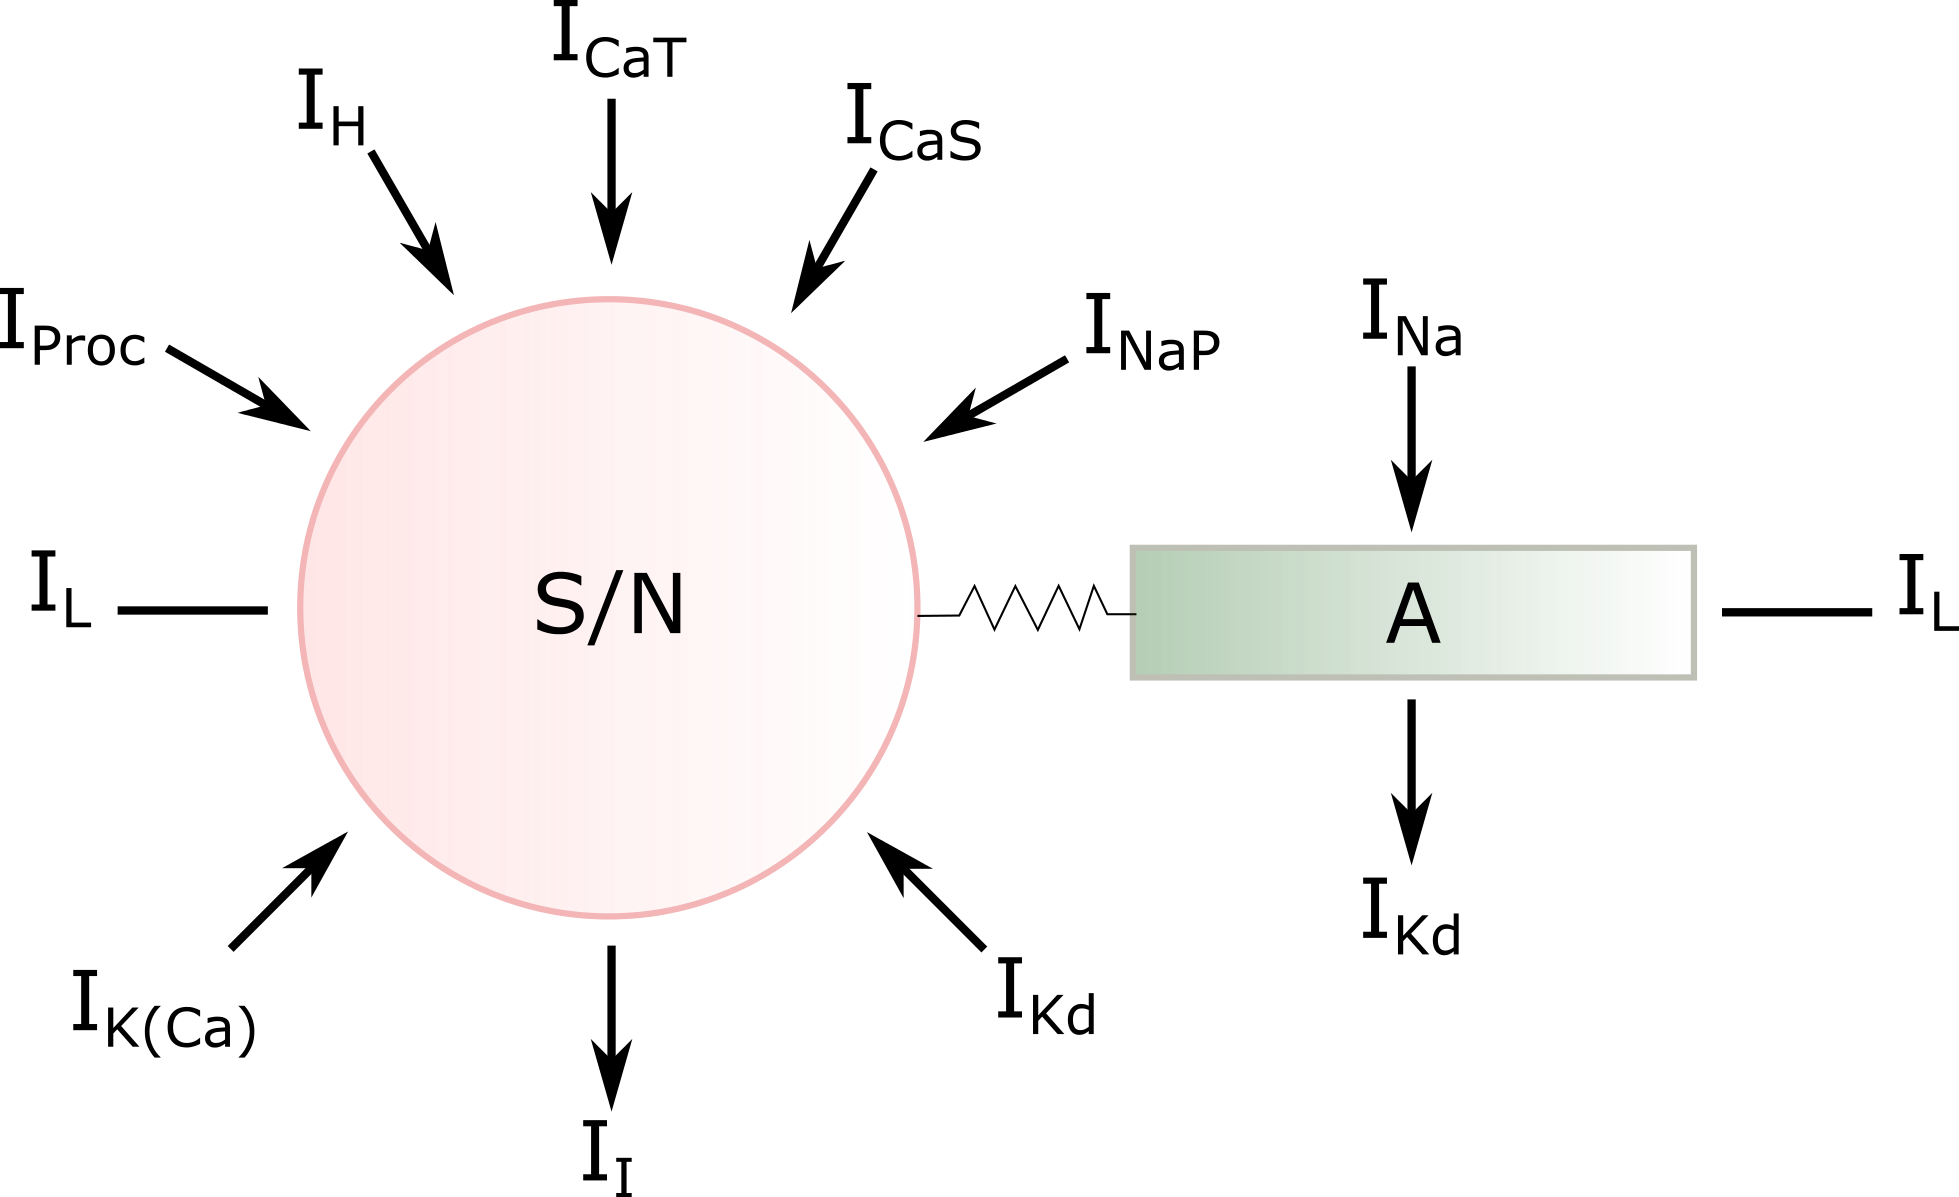
\includegraphics[width=8cm]{graphics/two_compartment.png}
		\caption[Two compartment model of a neuron.]{\textbf{Two compartment model of a neuron.} Each neuron is modelled with two compartments, S/N representing the soma and primary neurite and A representing the axon. }
		\label{fig:two_compartment}
	\end{center}
\end{figure}


\section{Parameters}
Parameters for the model was obtained from literature. For the \ac{AB} and \ac{PD} neurons the parameters were taken from research by Soto-Trevi\~{n}o \cite{Soto-Trevino2005}. The distinct intrinsic and dynamic properties of these two neurons were taken into account by using measurements from cultured \ac{STG} neurons in research performed by Turrigiano \textit{et al.} \cite{Turrigiano1995} The parameters for the \ac{LP} and \acp{PY} were adapted from Golowasch \textit{et al.} \cite{Golowasch1999a}.

\renewcommand{\tablename}{Table}
\begin{table}[H]
	\centering
	\tiny
	\caption{Parameter values of the model axons. Conductances ($g$) are in $mu S$ and reversal potentials ($E$) in $mV$.}
	\label{tab:modelparameters1}
	\begin{tabular}{ l l r l r l r l r}
		\hline
		\bf Channel & \multicolumn{2}{c}{\bf AB axon} & \multicolumn{2}{c}{\bf PD axon} & \multicolumn{2}{c}{\bf LP axon}& \multicolumn{2}{c}{\bf PY axon}\\ 
		\hline
		 & $g$ & $E$ & $g$ & $E$ & $g$ & $E$& $g$ & $E$\\ 
		\hline
		$I_{Na}$& $300e^{-3}$ & 50 \vline& $1,110e^{-3}$ & 50 \vline& $0.03e^{-3}$ & 20 \vline& $0.03e^{-3}$ & 20 \\ 
		$I_{K}$& $52.5e^{-3}$ & -80 \vline& $150e^{-3}$ & -80 \vline& $4e^{-3}$ & -80 \vline& $4e^{-3}$ & -80 \\
		$I_{L}$& $0.0018e^{-3}$ & -60 \vline& $0.00081e^{-3}$ & -55 \vline& $0.0075e^{-3}$ & -68\vline& $0.0075e^{-3}$ & -68\\
		\hline
	\end{tabular}
\end{table}

% Table generated by Excel2LaTeX from sheet 'Sheet1'
\begin{table}[H]
	\centering
	\tiny
	\caption{Parameter values of the model somas. Conductances ($g$) are in $/mu S$ and reversal potentials ($E$) in $mV$.}
	\label{tab:addlabel}%
	\begin{tabular}{llrlrlrlr}
		\hline
		\bf Channel & \multicolumn{2}{c}{\bf AB soma} & \multicolumn{2}{c}{\bf PD soma} & \multicolumn{2}{c}{\bf LP soma} & \multicolumn{2}{c}{\bf PY soma} \\
		 & g & e & g & e & g & e & g & e \\
		\hline
		$I_{Na}$  & $2.7e^{-3}$ & 50 \vline& $4.383^{-3}$ & 50 \vline& \centering\textemdash & \textemdash \vline& \textemdash & \textemdash \\
		$I_{H}$  & $0.054e^{-3}$ & -20 \vline& $0.219e^{-3}$ & -20 \vline& $0.005e^{-3}$ & -20 \vline& $0.005e^{-3}$ & -20 \\
		$I_{K}$  & $1890e^{-3}$ & -80 \vline& $1576.8e^{-3}$ & -80 \vline& $0.1e^{-3}$ & -80  \vline & $0.1e^{-3}$ & -80 \\
		$I_{KCA}$ & $6000e^{-3}$ & -80 \vline& $251.84e^{-3}$ & -80 \vline& \centering\textemdash & \textemdash \vline& \centering\textemdash &  \textemdash \\
		$I_{A}$  & $21.6e^{-3}$ & -80 \vline& $39.42e^{-3}$ & -80 \vline& $0.01e^{-e}$ & \textemdash \vline& $0.025e^{-3}$ & \textemdash \\
		$I_{P}$  & $570e^{-3}$ & 0 \vline& 0  & 0  \vline& $0.04e^{-3}$ & -10 \vline& 0  & -10 \\
		$I_{L}$  & $0.045e^{-3}$ & -50 \vline& $0.105e^{-3}$ & -55 \vline& $0.025e^{-3}$ & -68 \vline& $0.015e^{-3}$ & -68 \\
		$I_{CaT}$ & $55.2e^{3}$ & \textemdash \vline& $22.5e^{-3}$ & \textemdash \vline& \centering\textemdash & \textemdash \vline& \textemdash & \textemdash \\
		$I_{CaS}$ & $9e^{-3}$ & \textemdash \vline& $60e^{-3}$ & \textemdash \vline& \centering\textemdash & \vline & \textemdash & \textemdash \\
		$I_{Ca}$ & \centering\textemdash & \textemdash \vline& \centering\textemdash & \textemdash \vline& $0.1e^{-3}$ & 120 \vline& $0.1e^{-3}$ & 120 \\
		\hline
	\end{tabular}%
\end{table}%

\section{Equations}

Mathematically the currents for gap junctions ($I_{gap}$) and couplings between the S/N and A compartments are described with the same equation. Coupling currents in the coupled compartments are symmetric, thus the coupling current between the soma and the axon would be:

\begin{equation}
\label{eq:coup}
I_{axial_{S/N}} = -I_{axial_{A}}
\end{equation}

and the gap junction between neurons $i$ and $j$ would be:

\begin{equation}
\label{eq:gap}
I_{gap_{i}}=-I_{gap_{j}}
\end{equation}

For each of the S/N compartments the axial current is the product of the axial conductance and the difference of the membrane potential in the A and S/N compartments:

\begin{equation}
\label{eq:axial_conductance}
I_{axial_{S/N}} = g_{axial}(V_{S/N} - V_{A})
\end{equation}

Gap junctions use a similar equation where the conductance $I_{gap_{i}}$ is the product of the gap-junctional conductance and the membrane voltage difference between the two S/N compartments of neurons $i$ and $j$:

\begin{equation}
\label{eq:gap_conductance}
I_{gap_{i}} = g_{gap}(V_{S/N_{i}} - V_{S/N_{j}})
\end{equation}

In all compartments the conservation of current is represented by the partial differential equation of the form:

\begin{equation}
C\frac{dV}{dt} = I_{ext} - I_{int} - I_{coup}
\end{equation} 

and 

\begin{equation}
C\frac{dV}{dt} = I_{ext} - I_{int} - I_{gap}
\end{equation} 


where:

$C$ is the membrane capacitance.

$I_{ext}$ is the externally injected current.

$I_{int}$ is the sum of all modulatory and intrinsic currents.

$I_{coup}$ is the sum of the axial current of the adjacent compartment. 

$I_{gap}$ is the gap junctional current in the case of the S compartment.

Each of the currents is described in terms of maximal conductance and voltage-dependant gating variables:

\begin{equation}
I_{i} = g_{i}m_{i}^{pi}h_{i}^{qi}(V-E_{i})
\end{equation}

where:

$g_{i}$ is the maximal conductance.

$m_{i}$ is the activation current.

$h_{i}$ is the inactivation current.

$p_{i}$ and $q_{i}$ depends on the current type and takes integer values between zero and four.

$E_{i}$ is the reversal potential for ion ${i}$.

The behaviour of the activation and inactivation currents are modelled with the following equations:

\begin{equation}
	\label{eq:activation}
	\tau_{m}(V)\frac{dm}{dt} = m_{\infty}(V)-m
\end{equation}

\begin{equation}
	\label{eq:inactivation}
	\tau_{h}(V)\frac{dh}{dt}=h_{\infty}(V)-h
\end{equation}

where:

$m_{\infty}$ and $h_{\infty}$ are steady-state values.

$\tau_{m}$ and $\tau_{h}$ are time constants.

Table \ref{tab:gates} and \ref{tab:gates2} gives the dependency of voltage and intracellular $Ca^{2+}$ concentrations for each of these functions. The steady-state activation of $I_{KCa}$ is also dependent on $[Ca^{2+}]$ and provided in table \ref{tab:gates}.

The values of the exponents $p_{i}$ and $q_{i}$ are dependent on the current type and takes a value between 0 and 4.

The calcium activated potassium channels ($KCa$) of \ac{AB} and \ac{PD} are critical for their roles as pacemakers in the pyloric circuit. These channels only occur in the S/N compartments of the \ac{AB} and \ac{PD} and not in any of the other neurons. $Ca^{2+}$ is governed by the following equation:

\begin{equation}
\label{eq:KCa_concentration}
\tau_{Ca}\frac{d[Ca^2+]}{dt}-FI_{Ca}-[Ca^{2+}] + C_{0} 
\end{equation}

where:

$\tau_{Ca}$ is the $Ca^{2+}$ buffering time constant.

$C_{0}$ is the background intracellular $Ca^{2+}$ concentration.

$F$ converts the total $Ca^{2+}$ current $I_{Ca}$, in nA, into an intracellular concentration. 


The reversal potential for all currents, apart from $E_{Ca}$ are constants, given in table \ref{tab:modelparameters1}. The Nernst equation (\ref{eq:Nernst}) is used to compute the reversal potential for $E_{Ca}$, with an extracellular concentration of 13 $mM$ \cite{Buchholtz1992, Soto-Trevino2005}.

\begin{table}[H]
	\centering
	\caption{\ac{PD} and \ac{AB} voltage and calcium dependency for the steady-state activation $m$ and inactivation $h$ of the currents (adopted from \cite{Soto-Trevino2005} and \cite{Golowasch1999a})}
	\label{tab:gates}
	{\renewcommand{\arraystretch}{2}%
	\begin{tabular}{lcll}
		\hline
		& $m,h$ & $x_{\infty}$ & $\tau_{x}$,ms \\
		\hline
		% --- INa ---
		\multirow{3}{*}{ $I_{Na^{+}}$ } & $m^{3}$  & $\dfrac{1}{1+exp [ - ( V+24.7 / 5.29 ) ] }$ & $1.32 - \dfrac{1.26}{1+ exp \lbrack -( V+120 / 25 ) \rbrack}$ \\
		& $h$ & $\dfrac{1}{1 + exp [ ( V + 48.9 ) / 5.18 ]}$ & $ \Bigg\{ \dfrac{0.67}{1 + exp [ - ( V + 62.9 ) / 10] } \Bigg\} $ \\ 
		& & & $ \times \Bigg\{ 1.5 + \dfrac{1}{1 + exp [ ( V + 34.9 ) / 3.6 ] } \Bigg\} $ \\
		% --- IK ---
		$I_{K}$ & $m^{4}$ & $\dfrac{1}{ 1 + exp [ - ( V + 14.2 ) / 11.8 ]}$ & $7.2 - \dfrac{6.4}{ 1 + exp [ - ( V + 28.3 ) / 19.2] } $ \\
		% --- ICaT ---
		\multirow{3}{*}{ $ I_{CaT} $} & $m^{3}$ & $\dfrac{1}{ 1 + exp [ -( V + 25 ) / 7.2 ]}$ & $ 55 - \dfrac{49.5}{ 1 + exp [ - ( V + 48 ) / 17  ] } $ \\
		& $h$ & $ \dfrac{1}{ 1 + exp [ ( V + 36 ) / 7 ] } $ & AB:$ 87.5 - \dfrac{75}{ 1 + exp [ - ( V + 50 ) / 16.9 ] } $\\
		& & & PD:$ 350 - \dfrac{300}{ 1 + exp [ - ( V + 50 ) / 16.9] } $ \\
		% --- ICaS ---
		$ I_{CaS} $ & $ m^{3} $ & $ \dfrac{1}{ 1 + exp [ - ( V + 22) / 8.4 ] } $ & $ 16 - \dfrac{13.1}{ 1 + exp [ - ( V + 25.1 ) / 26.4 ] } $ \\
		% --- INap ---
		\multirow{2}{*}{ $ I_{Nap} $ } &  $ m^{3} $ & $ \dfrac{1}{ 1 + exp [ - ( V + 26.8 ) / 8.2 ] } $ & $ 19.8 - \dfrac{10.7}{ 1 + exp [ - (V + 26.5 ) / 8.6 ] } $ \\
		& $ h $ & $ \dfrac{1}{ 1 + exp [ ( V + 48.5 ) 4.8 ] } $ & $ 666 - \dfrac{379}{ 1 + exp [ - ( V + 33.6 ) / 11.7 ] }$ \\
		% --- h ---
		$ I_{h} $ & $ m $ & $ \dfrac{1}{ 1 + exp [ ( V + 70 ) / 6 ] } $ & $ 272 + \dfrac{1499}{ 1 + exp [ - ( V + 42.2 ) / 8.73 ] } $ \\
		% --- KCa ---
		% ----------- AB
		\multirow{2}{*}{ $I_{KCa}$ } & \multirow{2}{*}{ $m^{4}$ } & AB:$ \Bigg( \dfrac{ [ Ca ] }{ [ Ca ] + 30 } \Bigg) \times $ &  $ 90.3 - \dfrac{75.09}{ 1 + exp [ - ( V + 46 ) / 22.7] } $\\
		& & $\dfrac{1}{ 1 + exp [ - ( V + 51 ) / 4 ] } $ & \\
		% ----------- PD
		& & PD: $ \Bigg( \dfrac{ [ Ca ] }{ [ Ca ] + 30 }\Bigg) \times $ & \\
		& & $\dfrac{1}{ 1 + exp ([ - ( V + 51 ) / 8 ]) } $ & \\
		% --- IA ---
		\multirow{3}{*}{ $ I_{A} $ }& $ m^{3} $ (AB) & \multirow{2}{*}{$ \dfrac{1}{ 1 + exp [ - ( V + 27 ) / 8.7 ]}$} & \multirow{2}{*}{$ 11.6 - \dfrac{10.4}{ 1 + exp [ - ( V + 32.9 ) / 15.2 ] } $} \\
		& $m^{4}$ (PD) & &  \\
		& $h$ & $\dfrac{1}{ 1 + exp [ ( V + 45.9 ) / 4.9 ] } $ & $ 38.6 - \dfrac{29.2}{ 1 + exp [ - ( V + 38.9 ) / 26.5 ] }$ \\ 
		$I_{proc}$ & $m$ & $ \dfrac{1}{ 1 + exp [ - ( V + 12 ) / 3.05 ] }$ & $ 0.5 $ \\		
		\hline
	\end{tabular}
	}
\end{table}

\begin{table}[H]
	\centering
	\caption{\ac{LP} and \ac{PY} voltage and calcium dependency for the steady-state activation $m$ and inactivation $h$ of the currents (adopted from \cite{Golowasch1999a})}
	\label{tab:gates2}
	{\renewcommand{\arraystretch}{2}%
		\begin{tabular}{lcll}
		\hline
		& $m,h$ & $x_{\infty}$ & $\tau_{x}$,ms \\
		\hline
		% --- Ca ---
		\multirow{2}{*}{ $I_{Ca}$ } & $m$ & $\dfrac{1}{ 1 + exp [ 0.205 ( - 61.2 - V ) ] }$ & $ 30 + \dfrac{-5}{ 1 + exp [ 0.2 ( -65 - V ) ] } $ \\
		& $h$ & $\dfrac{1}{ 1 + exp [ -0.15 ( - 75 - V ) ] } $ & $ 150 $\\
		% --- K ---
		$I_{K}$ & $m$ & $ \dfrac{1}{ 1 + exp [ 0.1 ( -35 - V ) ] } $ & $ 2 + \dfrac{55}{ 1 + exp [ -0.125 (-54-V ) ] } $ \\
		% --- A ---
		\multirow{3}{*}{$I_{A}$} & \multirow{2}{*}{ $m$ } & PY:$ \dfrac{1}{1 + exp[ 0.2 ( -51 - V ) ] } $ & \multirow{2}{*}{$0.1$} \\
		& & LP: $\dfrac{1}{ 1 + exp [ 0.2 ( -60 - V ) ] } $ & \\
		& $h$ & $\dfrac{1}{ 1 + exp [ -0.18 ( -68 - V ) ] } $ & $50$ \\
		% --- P ---
		$I_{P}$ & $m$ & $ \dfrac{1}{1 + exp [ 0.2 ( -55 - V ) ] } $ & $6$ \\
		% --- Na ---
		\multirow{2}{*}{$I_{Na}$} & $m^{3}$ & $ \dfrac{1}{1 + exp[ 0.1 ( -42.5 - V ) ]} $ & $0.025$ \\
		& $h$ & $\dfrac{1}{1 + exp[ -0.13 * ( -50 - V ) ] } $ & $ \dfrac{10}{ 1 + exp [ 0.12 ( -77 - V ) ] } $ \\
		% ---Kd ---
		$I_{Kd} $ & $m^{4}$ & $ \dfrac{1}{ 1 + exp [ 0.2 ( -41 - V ) ] } $ & $ 12.2 + \dfrac{10.5}{1 + exp [ - .05 ( 58 - V ) ] } $ \\
		\hline
		\end{tabular}
	}
\end{table}

\subsection{Modelling the Impact of Dopamine}

\Ac{DA} differentially modulates the neurons of the pyloric network. The following combinations of variation to the $K^{+}$ channel conductances and gap junction conductances were modelled:

\begin{itemize}
\item The potassium conductances ($g_{K}$) for \acp{PY} were fixed to $10^{-4}$. Conductances for other channels were also all fixed. Gap junction conductances were varied from 0\% to 100\% of $2.7\times10^{-7}$ in increments of 10\%. 
\item Ten randomly generated potassium conductances in an initial range of $5\times10^{-5}$ to $0.2\times10^{-3}$ . Conductances of channels A and H were percentages of K (Table \ref{tab:percentages}). Gap junctions were modelled for each of the conductances at $10^{-6}$ at 100\%, 50\% and 10\%.
\item Ten randomly generated conductances in a narrower range of $9\times10^{-5}$ to $1.1\times10^{-4}$ . Conductances of channels A and H were percentages of K (Table \ref{tab:percentages}). Gap junctions were modelled for each of the conductances at $10^{-6}$, from 100\% to 0\%.
%\note{(Table \ref{tab:randomK1})}
%\item Ten randomly generated conductances in range ?. Other conductances fixed. Gap junctions at 10e-6, 50\% and 10\%
%\note{(Table \ref{tab:randomK2})}
\end{itemize}

\begin{table}{H}
	\centering
	\caption{Values for channels A and H were calculated as percentages of the potassium channels (\cite{Temporal2012})}
	{\renewcommand{\arraystretch}{2}%
	\begin{tabular}{l l}
		\hline
		\textbf{Channel conductance} & \textbf{Percentage (\%)} \\
		\hline
		gA & 0.8875 \\
		gH & 0.087 \\
		\hline
	\end{tabular}}
	\label{tab:percentages}
\end{table}

\subsection{Calculating Dyssynchrony}
\label{sec:dyssync}
After the models were run a \matlab script, findpeaks \footnote{http://terpconnect.umd.edu/~toh/spectrum/PeakFindingandMeasurement.htm}, was used to detect spikes for each of the modelled \acp{PY} (figure \ref{fig:findpeaks}). The detected spikes were then passed to another \matlab script, SPIKY \cite{Kreuz2013}\footnote{http://www.fi.isc.cnr.it/users/thomas.kreuz/Source-­‐Code/SPIKY.html.}. SPIKY uses the spike distance as a parameter-free and timescale-independent measure of spike train synchrony. SPIKY also calculates the inter-spike interval which quantifies local dissimilarities based on the neurons' firing rate profiles.  


\begin{figure}[H]
	\begin{center}
		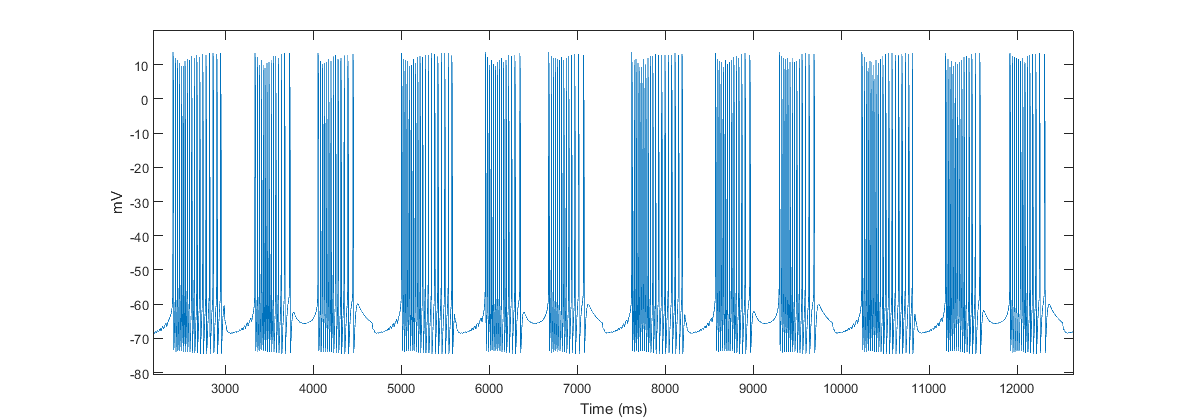
\includegraphics[width=\columnwidth]{graphics/peakfinder.png}
		\caption[findpeaks result.]{\textbf{findpeaks result.} findpeaks is a \matlab script that can detect spikes. The detected spikes are used by SPIKY to calculate spike-distance and inter-spike intervals. This plot was generated from the peaks detected by findpeaks from the output of the \matlab model. The trace represents one modelled \ac{PY} neuron. The peaks found for all the \ac{PY} neurons are passed to SPIKY which is then used to calculate \ac{ISI} and \ac{SD}}
		\label{fig:findpeaks}
	\end{center}
\end{figure}

In the next chapter the results of applying the methods discussed will be presented.

\

%\note{what is HH model
%how do you apply this to STG neurons
%where do you get parameters from - paper of ST, golowasch, harris-warrick
%how did yo get parameters py, lp, pd, ab, Temporal,
%how gap junctions model,
%how impact of da is model by changing gap junction strength.
%spiky
%}

\section{Results: The Model Output}

Traditionally \acp{PY} are modelled as one neuron implying that the same parameters are valid for all of them. However, we know that parameters vary quite widely and more recently it has also been shown that some conductance values maintain certain fixed ratios \cite{Temporal2012}. 

The variations and ratios of the parameters are implemented in our model as follows. A set of one hundred potassium conductance values were generated by using a uniform distribution over an interval. Each set consisted of five values (for the five \acp{PY}) randomly generated between of $5\times^{-5}$ to $2\times10^{-4}$. A and H channel conductances were calculated accordingly using the ratios as given in table \ref{tab:percentages}. For each of these sets, models were generated that would vary the gap junction conductance strength between zero and 100 percent of the gap junction normal strength ($10^{-6} \mu$Siemens).

For each of the models, the spike trains were detected using the \textit{findpeaks} \matlab script mentioned in section \ref{sec:dyssync}. The SPIKY \matlab script was then used to determine the \ac{ISI} and \ac{SD} for the five \ac{PY} spike trains (see figure \ref{fig:SpikeDistance}). The \ac{ISI} and \ac{SD} calculated by SPIKY are methods for quantifying the similarities in neuron's firing rate profiles and the degree of synchronisation between two spike trains on a continuous scale \cite{Kreuz2011}.

\begin{figure}[H]
	\begin{center}
		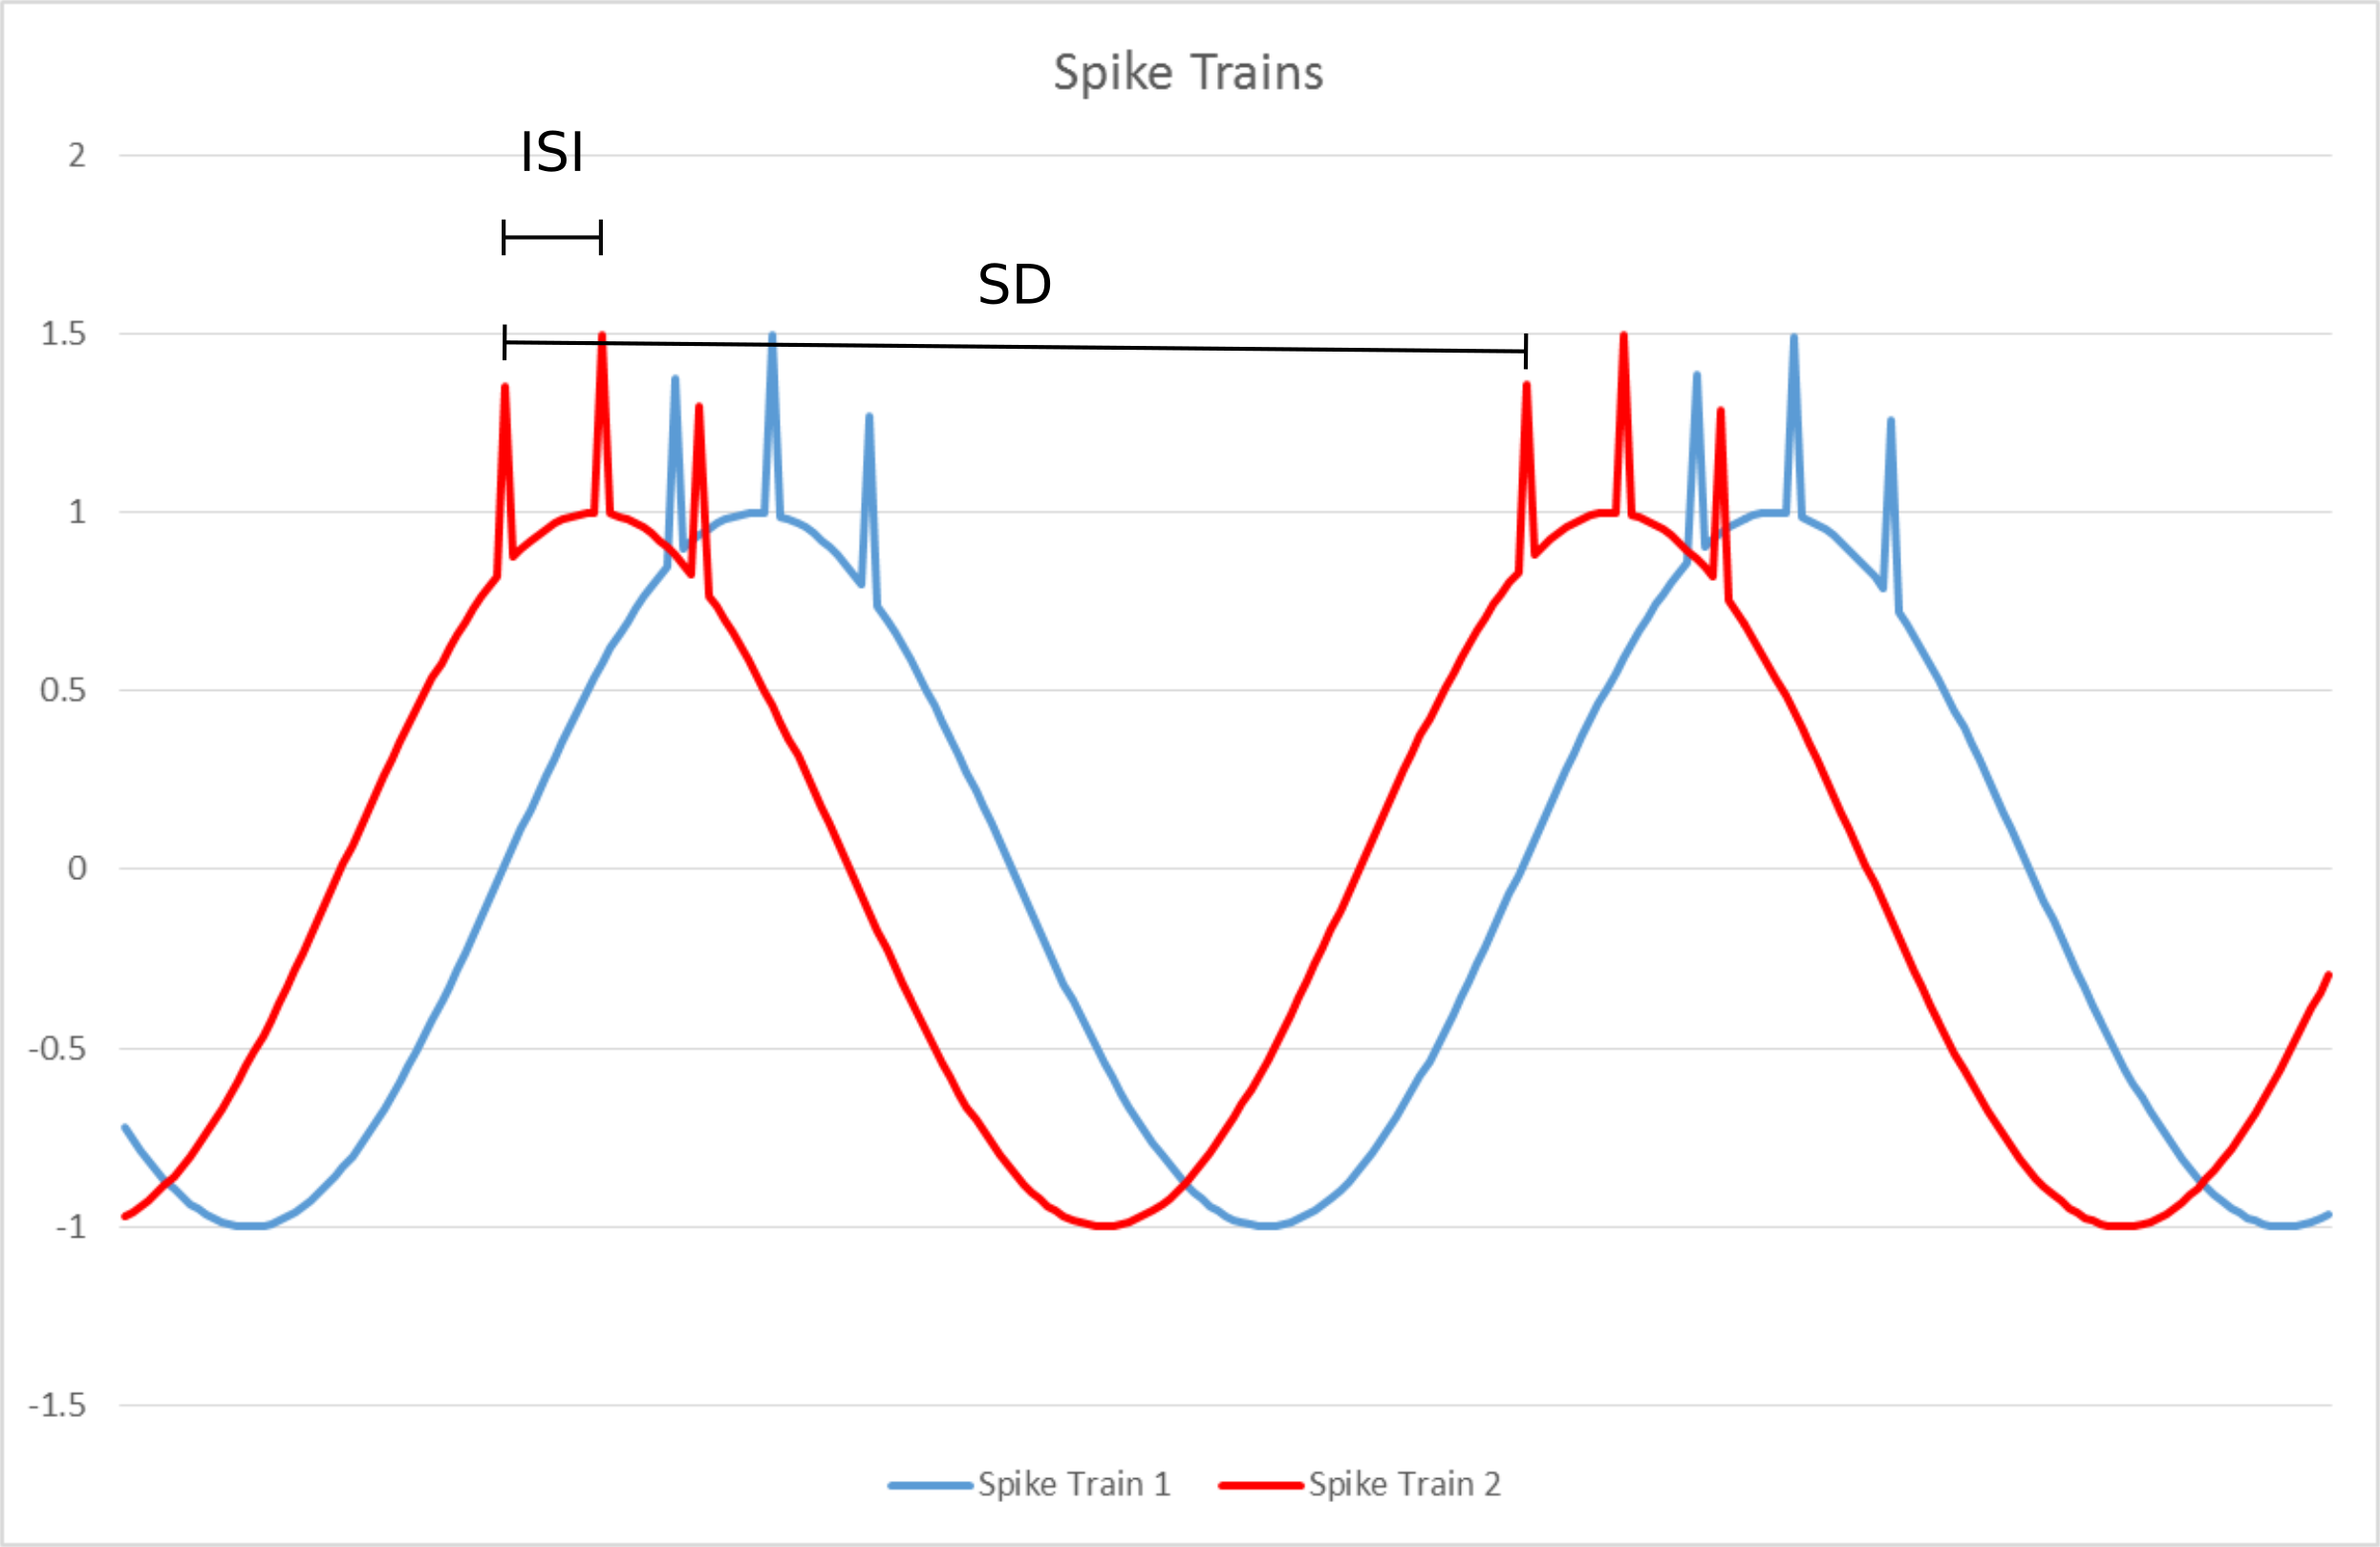
\includegraphics[width=\columnwidth]{graphics/SpikeDistance.png}
		\caption[Spike distance (SD) and inter-spike interval.]{\textbf{Spike distance (SD) and inter-spike interval.} A simplified representation of spike distance and inter-spike interval. ISI would be the distance between the spikes in a spike train. SD would be the distance between two spike trains. Detailed descriptions of exactly how these values are calculated by SPIKY can be found in the Kreuz papers \cite{Kreuz2007, Kreuz2009, Kreuz2011, Kreuz2013}}
		\label{fig:SpikeDistance}
	\end{center}
\end{figure}


Below are plots showing the effect of the changing gap junction strengths on \ac{ISI} and \ac{SD}. Figure \ref{fig:means_ISI} and \ref{fig:means_SD} plot the means of the \ac{ISI} and \ac{SD} values for each of the gap junction strength percentages. It would be expected that the stronger the gap junction conductances are, the closer the \ac{SD} would be to zero, thus more synchronised. The weaker the gap junction conductances are, the more de-synchronised the neurons are expected to be and thus the values \ac{SD} should increase. A changing \ac{ISI} indicates a change in the firing rate of a neuron.

To test the significance of any changes that might have occurred when the gap junction strength is changed, t-tests are used to test each gap junction conductance strength against the 100 percent strength. The \acp{ISI} and \acp{SD} were gathered and tested in this way for each gap junction conductance to provide a comparison measure. Figures \ref{fig:ttest_ISI} and \ref{fig:ttest_SD} show plots of the p-values from the t-tests over the gap junction strengths. The horizontal red line indicates a significance value of 0.05.

\begin{figure}[H]
	\begin{center}
		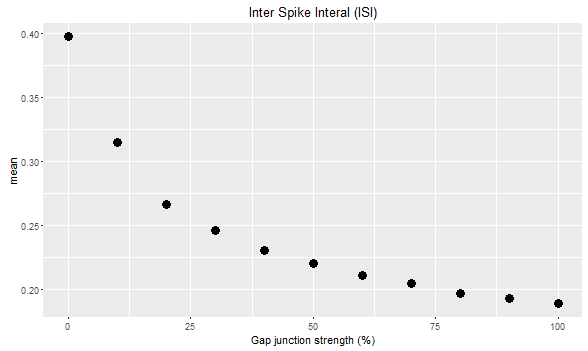
\includegraphics[width=14cm]{graphics/NewISImean.png}
		\caption[Means of inter-space interval for gap junction conductance strength.]{\textbf{Means of inter-space interval for gap junction conductance strength.}}
		\label{fig:means_ISI}
	\end{center}
\end{figure}
\begin{figure}[H]
	\begin{center}
		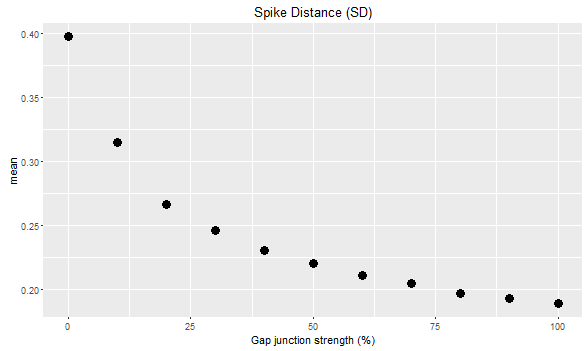
\includegraphics[width=14cm]{graphics/NewSDmean.png}
		\caption[Means of spike distance for gap junction conductance strength.]{\textbf{Means of spike distance for gap junction conductance strength.}}
		\label{fig:means_SD}
	\end{center}
\end{figure}

\begin{figure}[H]
	\begin{center}
		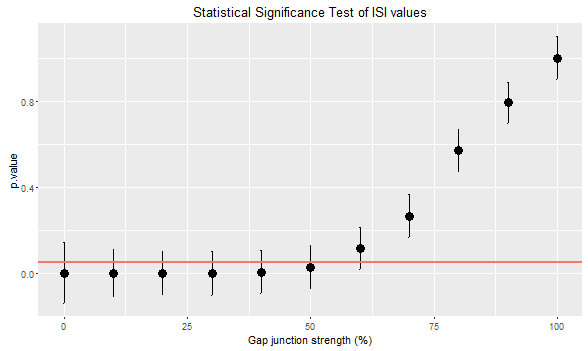
\includegraphics[width=14cm]{graphics/NewISIpvalue.png}
		\caption[Statistical Significance Test of ISI Values.]{\textbf{Statistical Significance Test of ISI Values.} The \ac{ISI} calculated for each gap junction conductance strength (from 0\% to 100\% of $10e^{-6}\mu$S) is tested against 100\% \ac{ISI}. The horizontal bars show standard deviation.}
		\label{fig:ttest_ISI}
	\end{center}
\end{figure}
\begin{figure}[H]
	\begin{center}
		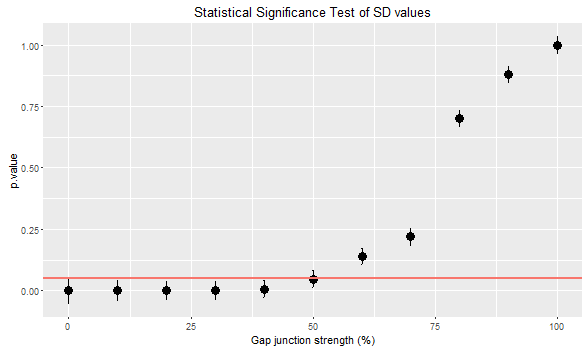
\includegraphics[width=14cm]{graphics/NewSDpvalue.png}
		\caption[Statistical Significance Test of Spike Distance Values.]{\textbf{Statistical Significance Test of Spike Distance Values.} The \ac{SD} calculated for each gap junction conductance strength (from 0\% to 100\% of $10e^{-6}\mu$ S) is tested against 100\% \ac{SD}. The horizontal bars show standard deviation.}
		\label{fig:ttest_SD}
	\end{center}
\end{figure}

\section{Conclusion}
This research investigated the possibility of accurately modelling the effect of dopamine on the pyloric central pattern generator circuit. Existing models only model two or three neurons at a time and groups neurons of the same type by representing them as one neuron. These models are unable to show the effect of modulation on the individual neurons of the same type and can thus not show any differential effects that might occur \cite{Soto-Trevino2005, Golowasch1999a}. The fact that neurons of the same type are modulated differentially can be seen in electrophysiological recordings and the challenge is to produce a model that could reflect such modulation.



The model built for this research is indeed able to reflect the de-synchronisation of the \acp{PY} that we observe in the biological system. The model included nine neurons, one \ac{AB}, one \ac{LP}, two \acp{PD} and five \acp{PY}. 

Although the effect of modulation on the whole pyloric network could not be observed, the necessary parameters for neurons other than the \acp{PY} are in place for further investigation. The model is also easily extensible to include parameters for more neurons and/or channels and junctions. The main problem still remains finding realistic parameter values for these parameters. 


\section{Discussion}
The main aim of this research was to develop a model that can accurately reflect the effect of neuromodulators on a neural network. The \ac{STG} of \species{Cancer pagurus} was selected because, as a well studied model system, it has been shown that all neurons and all synapses are differentially modulated. We are familiar with all the neurons in the system, as well as the complete connectome and all the neuromodulators that are found in the system. By implementing all known synapses and gap junctions as parameters to the model it is possible to vary the values. 

This is the first model to include all \ac{PY} and ac{PD} neurons, i.e. five \acp{PY} and two \acp{PD}, which makes it possible to show de-synchronisation that would occur under neuromodulatory conditions. 

The model showed that when gap junction strength was reduced, both the \ac{SD} and \ac{ISI} increased. The increasing \ac{SD} confirms the de-synchronisation of the \acp{PY}. Using a t-test it was possible to show that when the gap junction was reduced to 50 percent and less the increase of both the \ac{SD} and \ac{ISI} became statistically significant.  According to Harris-Warrick \cite{Harris-warrick1998}, \ac{DA} also decreases the cycle frequency of the pyloric rhythm. The increasing \ac{ISI} of the model could be the result of such a decreasing rhythm frequency.

What the model did not show conclusively is the decrease in the overall frequency of the pyloric rhythm under neuromodulatory conditions. The increasing \ac{SD} could be an indication of a changing frequency but since the model, at this point, is not reflecting modulation of neurons other than the \acp{PY} it is not possible to draw any conclusions with regards to the complete pyloric rhythm. An extended version of the model, that allows for the varying of parameters that reflect the effect of modulation of the rest of neurons, should be able to show altered rhythm frequencies.

Validation of the model is done by comparing its results to the quantified output of experimental \ac{VSD} data. How the experimental data was quantified is described in chapter \ref{chap:analysis}

\note{
Let's consider the following two terms for a moment:

\textit{\textbf{mathematics}, noun:} The science of space, number, quantity, and arrangement, whose methods involve logical reasoning and usually the use of symbolic notation, and which includes geometry, arithmetic, algebra, and analysis; mathematical operations or calculations (\textit{Oxford English Dictionary}). 

\textit{\textbf{model}, noun:} A simplified or idealized description or conception of a particular system, situation, or process, often in mathematical terms, that is put forward as a basis for theoretical or empirical understanding, or for calculations, predictions, etc.; a conceptual or mental representation of something (\textit{Oxford English Dictionary}).
}

The accuracy of a model relies to a great deal the numbers we provide to it as parameters. These number are most accurate if they are actually measured (rather than inferred or even guessed) and thus a great deal of time, in scientific research, is spent on improving our techniques of measurement. In neuroscience such methods often involve electrophysiology or even optogenetics and voltage sensitive dyes. Of importance to this research are methods of recording and quantifying neural activity in groups of neurons. However, not just measurements of neurons as a group but the contribution of each and every individual neuron in the group. 

The following chapter describes three methods that were investigated as possible, alternative or additional, methods for measuring the activity of large groups (i.e. more than four or five which is possible with traditions electrophysiological methods) of neurons at individual neuron level. In the first instance two newly developed voltage sensitive dyes were tested on the \ac{STG} and compared to existing dyes, in terms of toxicity and signal to noise level. The methods in chapter \ref{chap:Abstract} were used to quantify measurements for comparison to existing dyes. In the second instance the use of multi-electrodes on the \ac{STG} was investigated. The fact that \acp{MEA} are successfully used on other preparations do not guarantee that it will work on the crustacean \ac{STG} as the \ac{STG} presents its own sensitivities to being handled in the laboratory environment. Lastly, as a possible method for quickly injecting \ac{VSD} into multiple neurons, the use of a Picospritzer was investigated.